\documentclass{standalone}
\usepackage[latin1]{inputenc}
\usepackage{amsmath,amssymb,mathtools,mathrsfs}
\usepackage[T1]{fontenc}
\usepackage{tikz}
%\usepackage{amsthm}
%\usepackage[all]{xy}
%\usepackage{enumerate}
%\usepackage[hidelinks]{hyperref}

%\addtolength{\oddsidemargin}{-1cm}
%\addtolength{\evensidemargin}{-1cm}
%\addtolength{\textwidth}{2cm}
%\addtolength{\topmargin}{-2cm}
%\addtolength{\textheight}{2cm}


\date{\today}
\begin{document}
%\author{Florent Martin}

\title{}
%\maketitle
%\tableofcontents

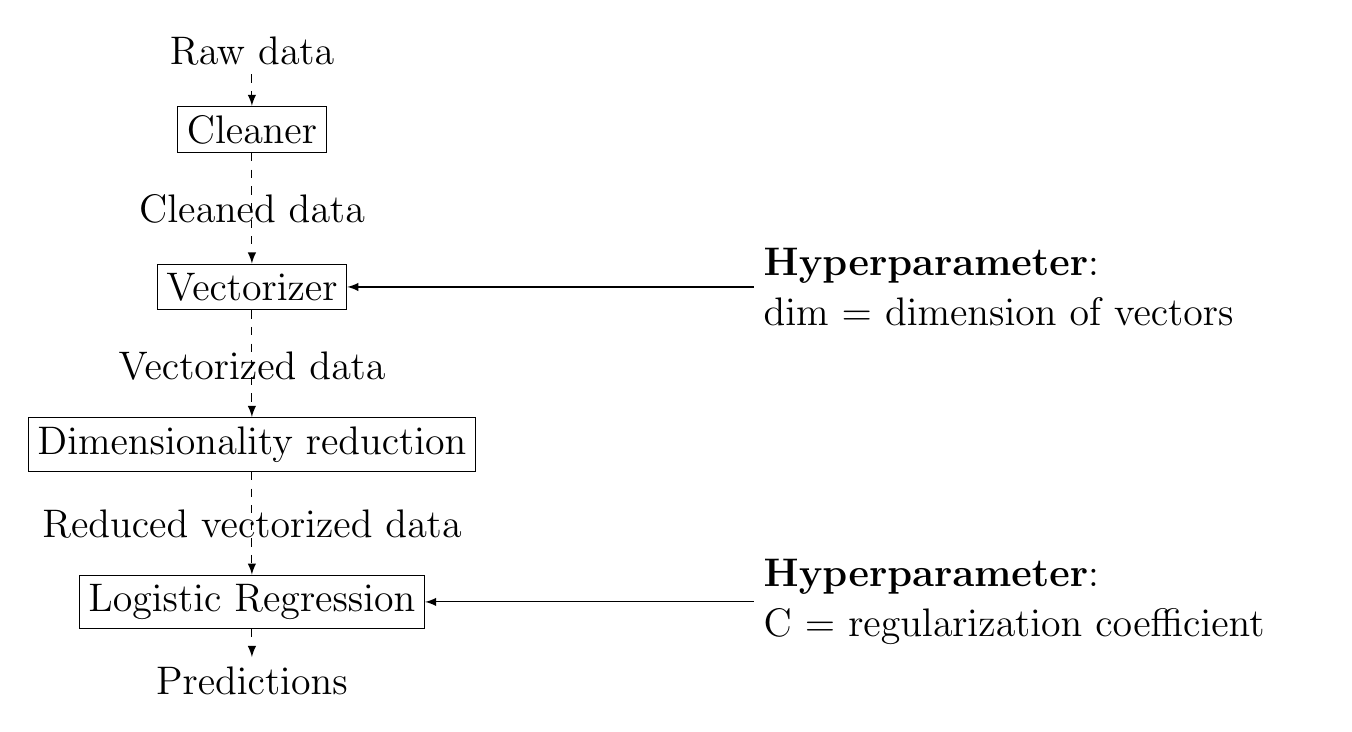
\begin{tikzpicture}

\tikzstyle{every node}=[font=\Large]


\pgfmathsetmacro\x{10}
\pgfmathsetmacro\y{0}

\node (raw) at (\x, \y) {Raw data};

\pgfmathsetmacro\y{\y-1}
\node[draw] (cleaner) at (\x, \y) {Cleaner};

\draw[->,>=latex,dashed] (raw) -- (cleaner);

\pgfmathsetmacro\y{\y-1}
\node (cleanded) at (\x, \y) {Cleaned data};

\pgfmathsetmacro\y{\y-1}
\node[draw] (vectorizer) at (\x,\y) {Vectorizer};

\node[text width=7cm] (hyperparameters_vec) at (\x + 10,\y) 
{{\bf Hyperparameter}: \\ 
dim = dimension of vectors };

\draw[<-, >=latex] (vectorizer) -- (hyperparameters_vec);

\draw[->,>=latex,dashed] (cleaner) -- (vectorizer);

\pgfmathsetmacro\y{\y-1}
\node (vecotorized) at (\x, \y) {Vectorized data};

\pgfmathsetmacro\y{\y-1}
\node[draw] (reducer) at (\x,\y) {Dimensionality reduction};

\draw[->,>=latex,dashed] (vectorizer) -- (reducer);

\pgfmathsetmacro\y{\y-1}
\node (reduced_vecotorized) at (\x, \y) {Reduced vectorized data};

\pgfmathsetmacro\y{\y-1}
\node[draw] (estimator) at (\x,\y) {Logistic Regression};

\node[text width=7cm] (hyperparameters_log) at (\x + 10,\y) 
{{\bf Hyperparameter}: \\ 
C = regularization coefficient };

\draw[<-, >=latex] (estimator) -- (hyperparameters_log);
\draw[->,>=latex,dashed] (reducer) -- (estimator);

\pgfmathsetmacro\y{\y-1}
\node (predictions) at (\x,\y) {Predictions};

\draw[->, >=latex, dashed] (estimator) -- (predictions); 


\end{tikzpicture}

%\bibliographystyle{plain}
%\bibliography{../../Articles/bibli}

\end{document}
